\documentclass[12pt,oneside,justify]{book}

\usepackage[utf8]{inputenc}
\usepackage{mathptmx}
\usepackage{geometry}
\usepackage{fancyhdr}
\usepackage{tocloft}
\usepackage{titlesec}
\usepackage{textcomp}
\usepackage{pdfpages} 
\usepackage{graphicx}
\usepackage[none]{hyphenat}
\graphicspath{ {images/} }
\usepackage[
backend=biber,
]{biblatex}  % irodalomjegyzék

\titleformat{\chapter}{\normalfont\huge}{\thechapter.}{20pt}{\huge} % egyedi chapter szöveg

\geometry{
	a4paper,
	lmargin=3cm,
	tmargin=3cm,
	bmargin=3cm,
	rmargin=2cm
}

\fancyhead
\fancyfoot
\pagestyle{plain} % oldalstílus
\pagenumbering{arabic} % oldalszámozás 

\renewcommand{\headrulewidth}{0pt}
\renewcommand{\contentsname}{Tartalomjegyzék} % tartalomjegyzék átnevezés
\renewcommand{\listfigurename}{Ábrajegyzék} % ábrajegyzék átnevezés
\renewcommand\cftchapaftersnum{.} % chapter szám utáni pont
\renewcommand\cftchapdotsep{\cftdotsep} % chapter, és irodalomjegyzék szöveg utáni pontok
\newcommand{\sectionbreak}{\clearpage} % címsorok új oldalon

\addbibresource{bibliography.bib}

% help section - to be deleted

% \chapter{Második bekezdés}
% \section{másik bekezdés 2 szintű}
% \subsection{First Subsection}
% \paragraph{az}

% Ezt idéztem \cite{AzureFundamentals}

% \noindent // bekezdés első sorának  nem indentálása

% end help section

\begin{document} 

\includepdf{outer_cover.pdf}
\includepdf{inner_cover.pdf}

\tableofcontents

\chapter{Virtualizáció}
\noindent Miért jó a virtualizáció. A virtualizált rendszerek előnyei. Modern virtualizációs megoldások
% \\TODO

\section{On-Premises rendszerek}

\subsection{Microsoft Hyper-V\texttrademark}

\subsubsection{Deduplikáció}
\noindent
A Microsoft a Windows Server 2012 szerver verzióban jelentette be a Deduplikációt. A deduplikáció az a folyamat amely feldolgozza az engedélyezett lemezek tartalmát és egyező adatblokkokat csak egyszer tárol le. Az ismétlődő blokkok esetén már csak referenciákat hagy. Ezzel a megoldással nagyon jó hatásfokkal lehet tárolóhelyet megtakarítani. A legjobban deduplikálható adatok a Virtualised Desktop Infrastructure - későbbiekben VDI rendszerek - amelyek esetén az operációs rendszer a hozzátartoztó frissítési csomagok, a feltelepített alkalmazások alapfileai többnyire minden rendszeren megegyeznek. Amennyiben a virtuális gépeken nagyon kevés egyedi file és telepített alkalmazás található úgy a deduplikációs ráta elérheti akár a 90\%-ot is.

%\\TODO kifejteni képekkel

\subsubsection{Virtual Network}

%\\TODO

\subsection{VMWare ESX \textsuperscript{\textregistered}}
\noindent

\subsection{Oracle\textsuperscript{\textregistered} VM}
\noindent

\section{Cloud megoldások}
\subsection{Microsoft Azure}
\noindent

\subsection{VMWare Cloud}
\noindent

\subsection{Oracle Cloud}
\noindent

\section{Platformok összehasonlítása}
\noindent

\chapter{Esettanulmány}
\section{Igényfelmérés}
\noindent

\section{Ajánlat}
\noindent

\section{Migráció cloudba}
\noindent

\chapter{Esettanulmány háttércég}

\section{Architektúra}

\noindent Architektúrális szempontból Intel alapú szervereket használtam. A fejlesztői és tesztelői környezet alapját 2 db Dell PowerEdge R710-es szerver adta. A szerverek a munka ideje alatt egyenként 2 db Intel{\textsuperscript{\textregistered}} Xeon{\textsuperscript{\textregistered}} E6545 processzorral (6 mag 12 HT szál), 96 GB DDR3 ECC RAM-al, 2x64 GB Rendszer lemezekkel illetve 2x136 GB adatlemezzel volt ellátva. A kettő szerver egy failover clusterben üzemelt. A rendszer és az adat lemezek RAID1-ben üzemeltek az adatvesztés megelőzése és a magas rendelkezésre állás biztosítása érdekében. Az adatlemezek mérete sosem volt gond a Windows Deduplikációs megoldása miatt.

\noindent
A rendszereinket központilag nem menedzselt, de egységes alapkonfigurációval látjuk el annak érdekében, ha az ügyfélnek segítségre lenne szüksége. 

\noindent
A megépített rendszerben használt alapkonfiguráció:
\begin{itemize}
	\item Processzor: 2 mag
	\item Memória: dinamikus memória 1 GB minimum, 2 GB induláskor, 4 GB maximum.
	\item Háttértár: 64 GB Operációs rendszer lemez, 32 GB Adat lemez
	\item Hálózati kártya: 1 DB a megrendelő rendszerinek a belső hálózatán
	\item Operációs rendszer: Windows Server 2012 R2
\end{itemize}

\subsubsection{A mester image használata}

\noindent A mester image előállítása nagyban meggyorsítja a megrendelt rendszerek üzembehelyezését. Alapvetően két nagy irányzatot lehet felismerni ezen megoldások terén. 

\noindent
Az első megoldás amikor már egy telljesen kész rendszert tartalmazó de syspreppelt virtuális merevlemezt másolunk át a konténer mappájába. Majd azt a virtuális gép konfigurációjakor becsatoljuk és már indítható is rendszer. Ezek után összesen a végfelhasználó szerződést kell elfogadnunk és már használatba is vehetjük a gépünket. Amelyet át kell nevezni, be kell állítani számára a megfelelő IP konfigurációt és már át is adható a felhasználónak. 

 
% \\TODO  A két irányzat alapvető lépéseit illetve a továbbiakban szükséges folyamatokat bemutatni
\begin{figure}[t]
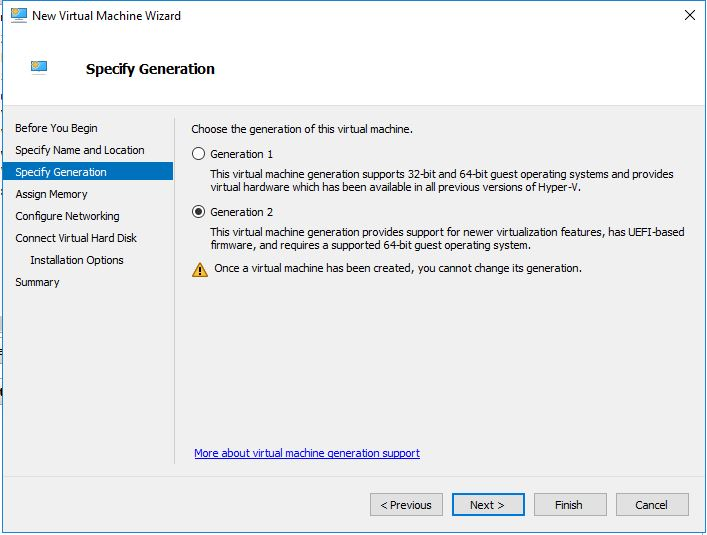
\includegraphics[width=0.8\textwidth]{generation_selection}
\caption{Generáció választás Hyper-V managerből készített virtuális gép esetén}
\label{fig:gen_selection}
\end{figure}


A másik irányzat amikor a Microsoft Deployment Toolkitet használjuk.

\section{Automatizált megoldások}
\noindent

\subsection{On-prem}
\noindent

Az automatizált rendszer első és lefontosabb építőköve a gyors virtális gépek elkészítése. Mivel az esettanulmányban egy szolgáltató céget tételeztem fel, így fontos volt, hogy minél kevesebb módon, lehetőleg telljesen automatikusan lehessen legyártani az igényelt virtális gépeket. 

\subsubsection{Provision-ObjectsForCompany.ps1}
Egy gyűjtő kód amely megfelelően paraméterezve elvégzni a telljes virtális gép létrehozás lépéseit. 
A következőkben taglalt scripteket hívja meg. 
A kódok végrehajtása az előkövetleményeknek megfelelően történik:
\begin{enumerate}
	\item VIrtuális Switch létrehozása ( Crete-NewVirtualSwitch.ps1 )
	\item Viruális gép(ek) létrehozása ( Create-VM.ps1 )
	\item A virtális gépek hálózatba fűzése ( Set-VMSwitchForVM.ps1 )
\end{enumerate}

% \\TODO

\subsubsection{Create-NewVirtualSwitch.ps1}

Virtuális switchek tulajdonságát korábban taglaltam. A cégnél a megrendelők rendszerei telljesen elválastott rendszerek, hacsak a megrendelők másképp nem rendelkeznek. Ellenben a virtális gépek amelyek egy megrendelőhöz kötődnek egymással közös hálózaton vannak. Szolgáltatói oldalon a cégekhez tartozó erőforrások azonosítása érdekében a megrendelő cég nevét eléfűzöm az erőforrás nevézhez. Amennyiben már létezik ilyen erőforrás úgy a script küld egy email üzenetet az üzemeltetőnek, hogy manuális ellenőrzésre van szükség.

% \\TODO ?

\subsubsection{Create-VM.ps1}

A script egy az argumentumaiban szereplő paramétereknek megfelelő VM konténert hoz létre. A beállításokat tekintve, ha valamelyik paraméter nincs felülbírálva az argumentumokban, akkor a korábban már taglalt alapbeállítás kerül felhasználásra.

A script úgy lett elkészítve, hogy képes felismerni, ha valamelyik lemez VHDX állománya már létezik.


% \\TODO




\subsubsection{Post-Configuration.ps1}
% \\TODO

\subsection{Cloud}
\noindent

\chapter{PowerShell}
\section{Történelme}
% \\TODO
\section{Programozási paradigmák}
% \\TODO

\addcontentsline{toc}{chapter}{\listfigurename}
\listoffigures
\printbibliography[heading=bibintoc,title={Irodalomjegyzék}]
\end{document}
